\documentclass[12pt,a4paper,onecolumn]{scrartcl}
\usepackage[utf8]{inputenc}
\usepackage{amsmath}
\usepackage{amsfonts}
\usepackage{amssymb}
\usepackage[ngerman]{babel}
\usepackage[left=2.5cm,right=2.5cm,top=2.5cm,bottom=2.5cm,head=14.5pt]{geometry}
\usepackage{scrlayer-scrpage} % Zur Anpassung der Kopf- und Fußzeilen
\usepackage{graphicx}
\usepackage{float}
\usepackage{lmodern}
\usepackage{mathtools}
\usepackage{graphicx}
\usepackage{grffile} % to allow underscores in filenames
\usepackage{subfig}
\usepackage{caption, booktabs}
\usepackage{paralist}
\usepackage[toc,acronym,nonumberlist,translate=babel]{glossaries}
\usepackage{underscore}
\usepackage{float}
\usepackage{wrapfig}
\usepackage{array}
\usepackage{adjustbox}
\usepackage{makecell}
\usepackage{pdfpages}
\usepackage{csquotes}
\usepackage{hyperref}
\usepackage{tabularx}
\usepackage{chngcntr} % Damit Zählungen von Abb und Co innerhalb sections mögl
%\usepackage[scaled]{uarial} % Schriftart
\usepackage{url}

\usepackage[backend=biber,natbib=true,hyperref=true,
			style=draft,maxnames=2,maxbibnames=2, isbn=false]{biblatex}
% STYLE draft SPÄTER NOCH GEGEN authoryear TAUSCHEN!!!!!!
\addbibresource{literatur.bib} %% Einbinden der bib-Datei
\DefineBibliographyStrings{ngerman}{
	andothers = {{et\,al\adddot}},}

\def\theequation{\thesection.\arabic{equation}} % Formeln beginnen mit Abschnittssnummer
\linespread{1.0} % Zeilenabstand
\pagestyle{scrheadings}
\clearpairofpagestyles % Löschen der Platzhalter
\counterwithin{figure}{section} % damit figure je section neu gezählt werden

\newcommand*\mytitle{Arbeitstitel: Eisenhypothese Dust-Event 2009}
\newcommand*\mysubtitle{Bachelorarbeit}
\newcommand*\myauthor{Marco Schulz}
\newcommand*\mydate{08.04.2021}
\newcommand{\cotwo}{CO\textsubscript{2}}

\begin{document}
\begin{titlepage}
\begin{center}
{\LARGE \textsc{\mysubtitle}} \bigskip \\
{\huge \textsf{\mytitle}} \bigskip \\
{\Large \myauthor \ - Matrikelnummer 7345692} \smallskip \\
{\Large Fassung vom \mydate} \bigskip \\
\begin{figure}[H]
\centering

\includegraphics[width=60mm]{bilder/unilogo.png}
\end{figure}
\bigskip
{\Large Institut für Geophysik und Meteorologie}
\bigskip
{\Large \\ Universität zu Köln}
\vspace{4cm}
\\
\end{center}
\begin{tabbing}
Erstgutachter: \quad  \= Prof. Yaping Shao (yshao@meteo.uni-koeln.de) \\[2ex]
Zweitgutachter:  \>  Dr. Hendrik Elbern (he@eurad.uni-koeln.de)
\end{tabbing}
\end{titlepage}
\setcounter{page}{2}
\ofoot{\pagemark}
\chead{{\small \mytitle}}
\automark{section}
\tableofcontents
\newpage
\begin{abstract}
DIESEN QUATSCH HABE ICH MIT DEM IPAD GESCHRIEBEN
Das kann ich erst am Ende schreiben!
\end{abstract}
\section{Einleitung}
Klima verändert sich. Aktuell Eiszeitalter. Glaziale, Interglaziale abwechselnd. Bekannt (aus Eisbohrkernen), dass geringe \cotwo -Konzentration in Atmosphäre während Glazialen. Deckt sich mit den geringen Temperaturen. Wohin das ganze \cotwo ? Phytoplankton sorgt für $50\%$ des jährlichen \cotwo -Austauschs \citep{Field.1998} und erzeugen etwa 45 gt organischen Kohlenstoff pro Jahr \citep{Falkowski.1998}. Phytoplankton benötigt \cotwo \ zum Wachsen, wodurch dieses zu Biomasse konvertiert wird. Somit bei erhöhten Phytoplankton weniger \cotwo . Warum wächst Phytoplankton dann nicht beständig, bis alles \cotwo\ aufgebraucht? Weitere limitierende Faktoren, da zur Fotosynthese weitere Nährstoffe benötigt werden. Nitrat und Phosphate als Nährstoffe, auch von Tiefsee. \citet{Martin.1988} zeigen, dass Eisen limitierender Faktor. Eiseneintrag hauptsächlich aus Staub. Wenige Staubquellen in Südhemisphäre bzw. südl. Ozean (vgl. China/Sahara). Dadurch Eisenmangel, hingegen reich an Nitraten und Phosphaten aufgrund Upwelling (aufgrund Ekmantransport der zyklonalen Zirkumpolarströmung). Falls dann doch größere Eisendeposition, Phytoplankton-Blüten. Dies als mögliche Erklärung für geringe \cotwo - Konzentrationen während Glazialen (Modelle zeigen, dass dies ungefähr die Hälfte des \cotwo \ Rückgangs erklären könnte. Etwa 16 gt Kohlenstoff werden aktuell pro Jahr durch die biologische Pumpe im Ozean archiviert \citep{Falkowski.1998}. Wenn diese Hypothese angenommen, dann bei größeren Staub-Events (kleine Zeitskala) vermehrtes Phytoplankton Wachstum wahrscheinlich. Ein großes Event 2009 in Australien. Dieses soll in dieser Arbeit genauer untersucht werden. Abgleich Staub- bzw. Eisendeposition mit Entwicklung Phytoplankton (bzw. Chlorophyll-$\alpha$). Dazu benutze Kölner WRF-Staub-Weiterentwicklung. Vergleich mit Satellitenbildern. Nutze verschiedene Verfahren der Statistik. Berücksichtige Ozeanzirkulation und Wind. Falls Zusammenhang gezeigt werden kann dann Hypothese wahrscheinlich. Wäre weiteres Indiz für Eisenhypothese. Wurde schonmal gemacht \citep{Gabric.2016}. Prüfung des Kölner Modells. Zusammenhang $\Rightarrow$ ggf. ebenfalls Hinweis dass Modell gut.
\section{Gabric.2016}

\begin{itemize}
\item Tasman Sea $25^\circ$ S bis $40^\circ$ S Untersuchungsareal
\item data: Chl + aeorosol optical depth (AOD)
\begin{itemize}
\item chl data: dialy + 8 day MODIS-AQUA
\item AOD data: 550 nm, 4km resolution 
\end{itemize}
\item divided into $5^\circ$ lattitude band
\item DVR kumulativ
\item Hovmoller Plots (x: zeit, y: latidude, longitude)
\item cloud processing / wet deposition wichtig
\item Response hauptsächlich südlich der tasmanischen Front ($\approx 32^\circ$ S) 
\item Staubdeposition weiter im Norden

\end{itemize}

\section{Theorie}
\subsection{Kohlendioxid und Klima}
\subsection{Wachstum von Phytoplankton}
Kurz: Welcher Prozess passiert genau bei Nährstoffe $\Rightarrow$ Phytoplankton / Fotosynthese \\\\
Phytoplankton sind Einzeller.
Wachstumsbeeinflussende Faktoren sind \citep{Falkowski.1998}):
\begin{enumerate}
\item mixed-layer depth
\item nutrient fluxes
\begin{enumerate}
\item Phospor \citep{REDFIELD.1960}
\end{enumerate}
\item food-web structure
\end{enumerate}
\citet{Boyce.2010} folgern, dass der Reichtum an Phytoplankton insgesamt seit Beginn der Messungen (1899) aufgrund der Erwärmung der Ozeane abgenommen hat. Es wird geschätzt, dass das globale Median jährlich um etwa 1\% abnimmt. Da die Klimamodelle steigende (Meeres-)Temperaturen prognostizieren ist es wahrscheinlich und problematisch, dass die Menge an Phytoplankton, der Basis aller Nahrungsketten im Ozean, zukünftig noch weiter abnimmt \citep{Siegel.2010}. Klimaänderungen werden direkt (andere Ozeanchemie) und indirekt (Änderungen in der Ozeanzirkulation) die Verteilung des Phytoplanktons verändern \citep{Falkowski.1998}. Mithilfe Temperatur des Oberflächenwassers, einfallender Sonnenstrahlung, mixed-layer-depth, Up- und Downwellingzonen kann aus CHL-a Konzentration die NPP abgeleitet werden \citep{Falkowski.1998}. Für Kieselalgen ist Zufuhr von Kieselsäure essenziell; diese tritt fast ausschließlich südlich der Südpolarfront auf \citep{Falkowski.1998}.
\\\\
elemental composition of phytoplankton (106C/16N/1P) \citep{Falkowski.1998}

\subsection{Eisenhypothese}
Andere Nährstoffe für Phytoplankton können durch aufsteigendes Tiefenwasser bereitgestellt werden. Eisen und Mangan werden hingegen hauptsächlich durch äolischen Staub eingebracht. Verweildauer von etwa 6 Monaten in oberflächennahem Wasser bis ca. 150m Tiefe \citep{Hayes.2015}. Nitrogenase (Enzymkomplex) kann N$_2$ reduzieren und Stickstoff somit biologisch verfügbar machen. Nitrogenase selbst benötigt (bzw. besteht aus) Eisen. Meistens Trichdesmiumspp., das N$_2$ bindet \citep{Falkowski.1998}.
\\\\ Insbesondere im südlichen Ozean kann auch Mangan limitierender Faktor sein \citep{Browning.2021}. Untersuchungen von Eisbohrkernen zeigen, dass Eisenzufuhr durch äolischen Staub in glazialen Perioden um eine Größenordnung größer war als in Interglazialen \citep{Falkowski.1998}.
\begin{figure}[ht]
\centering
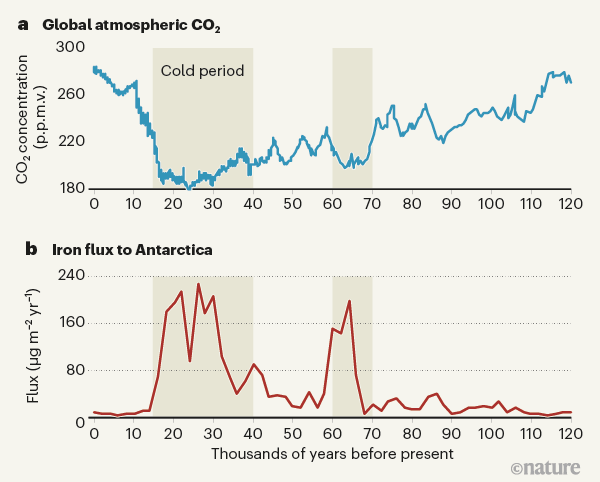
\includegraphics[width=0.7\textwidth]{bilder/Stoll2020/antarctic-iron-global-co2.png}
\caption{Antikorrelation von \textbf{a} globaler \cotwo \ Konzentration und \textbf{b} Eisendeposition in der Antarktis \citep{Stoll.2020}}
\end{figure}
\subsubsection{Düngung funktioniert nicht}
verschiedene Ursachen. Verweilzeit in Oberflächenwasser \citep{Hayes.2015}. Aufnahmefähigkeit / Rezeptivität ist saisonal variabel \citep{Gabric.2016}, Sekundärquelle. In nährstoffarmen Gewässern haben extrem kleine Phytoplankton-Organisamen bei der Verarbeitung von Nährstoffen (Exkrementen der Verbraucher) einen Wettbewerbsvorteil, da großes Oberflächen zu Volumen- Verhältnis \citep{Falkowski.1998}.Wenn hingegen \textit{neue} Nährstoffe bspw. durch Upwelling nach oben gelangen, hat größeres Phytoplankton, insbesondere Kieselalgen einen Wettbewerbsvorteil (aufgrund Vakuole, schnellere Aufahme). Das Plankton, das sich wiederum von diesen ernährt, ist typischerweise größer, benötigt für Entwicklung (Larvenstadium) mehr Zeit; dadurch im gegensatz zu obigen Arealen Blooms möglich und stärkere biologische Pumpe. \citep{Falkowski.1998}. Zeitreihen für Messungen der Ozeanbiologie sind im Vergleich zu Land sehr kurz, wodurch Schätzen auch unzuverlässiger sein können \citep{Falkowski.1998}. Häufigste Beschränkung ist durch Verfügbarkeit von gebundenem anorganischem Stickstoff \citep{Falkowski.1998}.
\subsubsection{Biologische Pumpe}
Niedriger Sauerstoffgehalt in der Tiefsee weist auf starke biologische Pumpe hin (dortige durch mehr absinkendes Plankton angereicherte Organismen verbrauchen mehr Sauerstoff?). Im aktuellen Ozean beträgt der (Sink)Fluss ca. 16 Pg Kohlenstoff pro Jahr \citep{Falkowski.1998}. In Küstengebieten (Upwelling) sehr deutlich $\Rightarrow$ Fischerei profitiert. Hoher Sauerstoffgehalt führt zu oxidiertem Eisen; oxidiertes Eisen ist nicht löslich und sinkt $\Rightarrow$ geringer Eisengehalt \citep{Falkowski.1998}


\subsection{Staubkreislauf}
Wichtige Verbindung zu Energie- und Kohlenstoffkreislauf \citep{Shao.2011} - Staub entstammt nicht nur ariden Wüstengebieten. Ein nennenswerter Anteil ($>$ 5\%) entsteht in kalten/glazialen Regionen hauptsächlich durch die Bewegungen von Gletschermassen und den damit verbundenen Abreibungen. Verwitterungsprozesse spielen im Gegensatz zu ariden Gebieten eine untergeordnete Rolle \citep{Marx.2018}. -
\subsubsection{Staubquellen in Australien}
Staub, der \textit{später} emittiert wird, entstammt häufig einem anderen Ort als dem der Emission. Diese sind i.d.R. benachbarte Regionen höherer Feuchte, in denen chemische und physikalische Verwitterung stattfindet. Während des Transports zur Region der Emission wird die Partikelgröße weiter reduziert (zermahlen, separieren)\citep{Marx.2018}. - größte Teil Zentralaustralien \citep{Shao.2011} siehe auch Lake Eyre basin. \\\\
Laut \citet{Deckker.2019} sind \textit{Kati Thanda-Lake Eyre} Region und \textit{Darling Riverine Plain} (Oberlauf des Darling River) Hauptquellen. Der Kontinent deckt insgesamt ein breites Spektrum an Oberflächengeologie ab, sehr alte Landmasse; einige Flächen sind mehr als 2.5 Milliarden Jahre alt (aus dem Archean). Durch die Besiedelung und Landnutzung durch den Menschen haben sich signifikante Änderungen ergeben, die bis 1945 mutmaßlich zu einer höheren Frequenz an Staubstürmen geführt haben. Nach verbesserter Landnutzung nahmen auch die Staubstürme wieder ab \citep{Deckker.2019}. Vgl. größte Staubereignisse vor 2009 waren in den 1940'ern.
\subsubsection{Eisen in Staub}
Nicht jede Form von Eisen kann als Dünger dienen. Muss entsprechend gelöstes (?) Eisen sein. Transportprozesse und Wolkenbildungen können die Transformation zu diesem tauglichen Eisen fördern \citep{Shao.2011}. Die Planktonart Trichodesmium kann die Rate des Eisenauflösens von Oxiden und Staub beschleunigen (im Gegensatz zu anderem Phytoplankton) \citep{Gabric.2016}. In Sediment enthält Staub häufig die Fe$^{3+}$ Minerale Hämatit und Goethit \citep{Reynolds.2014}.
\begin{table}[H]
\begin{tabularx}{\textwidth}{X X l}
		\toprule
			\thead{Eisenoxid(hydrate)} & \thead{Verhältnisformel} &  \thead{Vorkommen} \\	
		\midrule
		Hämatit & Fe$_2$O$_3$ & Mineral, trigonales Kristallsystem \\
		Maghemit & Fe$_2$O$_3$ & Mineral, kubisches Kristallsystem \\
		Magnetit & Fe$_2$O$_4$ & Mineral, kubisches Kristallsystem \\
		Goethit & $\alpha$-Fe$^{3+}$O(OH) & Mineral, orthorhombisches Kristallsystem \\		
		\bottomrule
\end{tabularx}
\caption{Beschreibung} \label{table:eisenoxid}
\end{table}
\subsubsection{Emissions- und Depositionsmodelle}
ggf. lieber in Kapitel Methoden
\subsection{Wind und Oberflächenströmungen}
Verkleinerung der Tiefe der Oceanic Mixed Layer von September auf Oktober \citep{Tilburg.2002} (abchecken, dass der Bloom nicht daher kommt!). Einteilung in \textit{nördlich der Tasmanischen Front} und \textit{südlich der tasmanischen Front}? Phytoplanktonproduktion hängt von Up- und downwelling-Prozessen durch mesoskalige Wirbel ab \citep{Tilburg.2002} $\Rightarrow$ Vorticity der Ozeanströmungen berechnen?Besser sea surface height (SSH) Anonmalien angucken. Was, wenn Blüte bei \citet{Gabric.2016} aufgrund von tieferen mixed-layer aufgrund des Sturms? $\Rightarrow$ Winddaten vergleichen. 
\section{Beschreibung des Staubsturms in September 2009}
stärkstes (in Bezug auf Sichtweitenreduzierung) Staubevent über Sydney seit es verlässliche Aufzeichnungen gibt (1940, \citet{Leys.2011}). Staubstürme üblich im ariden Inland. Vorangegangen sind Monate und Jahre mit im Vergleich zum Durchschnitt höheren Temperaturen und unterdurchschnittlichem Niederschlag; dadurch schwache Vegetation und trockene Erdböden \citep{Leys.2011}.
\section{Wetter}

\section{Staubtransport}
Staubquellen gemäß \citep{Leys.2011} 
\begin{enumerate}
\item lower Lake Eyre Basin
\item grazing lands of north western NSW
\item mining areas around Cobar und Broken Hill
\item Channel Country of western Queensland
\end{enumerate}



\section{Methoden}
hole Zeitreihe Chlorophyll alpha Entwicklung von September bis Oktober (bzw. falls saisonale Veränderung, den Zeitraum, welcher der Kurve Dust-Event-Zeitraums entspricht) gemittelt über bspw. 10 Jahre. Berechne daraus Anomalie 2009 und vergleiche diese mit Staubdeposition.
\subsection{iron residence time modell}
\subsection{phytoplankton response time modell}
turn-over time ist von Größenordnung einer Woche oder weniger \citep{Falkowski.1998}: abgeleitet durch: 45 bis 50 Pg Kohlenstoff produzieren Phytoplankton pro Jahr, aktuell im Ozean sind aber immer nur ca. 1 Pg, das heißt dass das jeweils aktuelle Phytoplankton immer nach ca. einer Woche \textit{umgesetzt} wurde.

\subsection{WRF Modell}
nur kurze Vorstellung, da grundsätzlich nur der Output verwendet werden soll. Vergleich mit von \cite{Gabric.2016} genutzem Modell CEMSYS
\begin{table}[H]
\begin{tabularx}{\textwidth}{X X}
		\toprule
			\thead{Kategorie} & \thead{Größe}\\
		\midrule
		1 & $0.5 \ \mu$m effektiver Radius \\
		2 & $1.4 \ \mu$m effektiver Radius \\
		3 & $2.4 \ \mu$m effektiver Radius \\
		4 & $4.5 \ \mu$m effektiver Radius \\
		5 & $8.0 \ \mu$m effektiver Radius \\
		\bottomrule
\end{tabularx}
\caption{Die Staubpartikel wurden in verschiedene Korngrößen unterteilt} \label{table:binsizes}
\end{table}
\subsubsection{Emissions Schema}
Zur Modellierung der Staubemissionen wurde das Schema von \citet{Shao.2004} verwendet und in WRF implementiert. Als Auslöser für Emissionen werden grundsätzlich zwei Mechanismen erwogen: Beschuss durch Salz und der Zerfall von Aggregaten. Zusammengefasst setzt sich das Emissionsschema \citep{Shao.2004} aus folgenden Gleichungen zusammen:
\begin{align}
\tilde{F} (d_i,d_s) &= c_y \eta_{fi} \left[\left(1-\gamma\right) + \gamma
\sigma_p \right] \left(1+\sigma_m \right) \frac{g \cdot Q}{u^2_*} \\
\gamma &= \exp \left[-\left(u_* - u_{*t} \right)^3\right] \\ 
\sigma_m &= 12 \cdot u_*^2 \frac{\rho_b}{p} \left(1 +14 \cdot u_* \sqrt{\frac{\rho_b}{p}} \right)
\end{align}
Dabei ist $\tilde{F}(d_i,d_s)$ die Emissionsrate für die Staubpartikelgröße $d_i$ und das Salz der Partikelgröße $d_s$; $c_y$ ein dimensionsloser Koeffizient; $\eta_{fi}$ der Anteil des insgesamt emittierbaren Staubs; $\sigma_p = \frac{\eta_{mi}}{\eta_{fi}} = \frac{p_{m}(d_i)}{p_{f}(d_i)}$ das Verhältnis zwischen der Massenverteilung freien Staubs $\eta_{mi}$ zu der des ingesamt emissionsfähigen Staubs $\eta_{fi}$ pro Einheitsbodenmasse für die Partikelgrößenklasse $i$ bzw. den entsprechenden Verteilungen für die Partikelgrößenverteilungen $p_{m}(d_i)$ und $p_{f}(d_i)$;  $\sigma_m= \frac{m_\Omega}{m}$ das Verhältnis zwischen der Masse  $m$ des einschlagenden Partikels und der durch \textit{Bombardement} ausgeworfenen Masse $m_\Omega$; $g$ die Erdschwerebeschleunigung; $Q$ der stromweise Salzfluss; $u_*^2$ die Reibungsgeschwindigkeit; $u_{*t}^2$ der Schwellenwert für die Reibungsgeschwindigkeit; $\rho_b$ die Bodenschüttdichte und $p$ der plastische Bodendruck.
\subsection{Phytoplankton}
Climate Data Store \nocite{*}
\\\\
Messungen des Chlorphyll-$\alpha$ geben Rückschluss auf Phytoplankton \citep{RYTHER.1957}(muss ich noch lesen)

\subsection{EOF?}
\subsection{Riegers Principal Components?}

\section{Auswertung und Diskussion}
\subsection{Anpassungen nach der ersten Simulation}
Die Ergebnisse der WRF-Simulation sollten in einem ersten Schritt durch eine grobe Übersicht auf Plausibilität, d.h. der wahrscheinlichen Abweichung von der Realität überprüft werden. Da ein relativ langer Zeitraum von 12 Tagen simuliert wird, sind auch größere Abweichungen wahrscheinlich. Ganz allgemein sind Wetterprognosen i.d.R. nur für die ersten Tage wirklich präzise. Die Wahrscheinlichkeit, dass das berechnete Wetter eintritt nimmt dann aufgrund des chaotischen Verhaltens der Atmosphäre und den beschränkt zur Verfügung stehenden diskreten Startwerten stark ab \textbf{(Quelle ergänzen)}. Beobachtungs- bzw. Reanalysedaten werden dem Modell zum Startzeitpunkt und an den Rändern geliefert. Die Zustände der zeitlich und räumlich dazwischen liegenden Gitterpunkte sind dann (ausschließlich) vom Modell simuliert (\textbf{Quelle Sven, nochmal checken}). Für den Großteil des untersuchten Gebietes liegen ohnehin keine Beobachtungsdaten vor. Der australische Kontinent ist relativ dünn mit Wetterstationen besetzt und Beobachtungen durch Satelliten sind hinsichtlich  zeitlicher und räumlicher Auflösung ebenfalls häufig relativ grob. Darüber hinaus können die interessanten Parameter meist nur indirekt ermittelt werden. 
\\

Dennoch können einfache Vergleiche einen ersten Eindruck von der Qualität der Simulation vermitteln. Hierzu wurden die simulierten Staubkonzentrationen und Emissionen mit Satellitenbildern, Beobachtungsdaten und Schätzungen aus der diesbezüglichen Literatur verglichen. Der Abgleich mit den (Echt-Farben-) Satellitenbildern zeigt, dass die Fortbewegung und Ausdehnung der Staubwolke vom Modell grundsätzlich erfasst wird. Auf Abbildung \ref{fig:wrf_sat} ist jedoch ebenfalls gut sichtbar, dass das Modell zu späteren Zeiten eine deutlich höhere Staubkonzentration im Nordwesten Australiens simuliert, als von den Satellitenbildern direkt ableitbar wäre. Dabei ist zu beachten, dass die (Echt-Farben-) Satellitenbilder keine direkten Rückschlüsse auf die Staubkonzentration zulassen. Es können durchaus höhere Staubkonzentrationen vorliegen, die auf Satellitenbildern nicht erkannt werden können (\textbf{Behauptung Shao, Quelle ergänzen}). Aufgrund der dort simulierten sehr hohen Konzentrationen wird allerdings vermutet, dass entsprechende Emissionen überschätzt werden.

\begin{figure}[H]
	\begin{minipage}[c]{0.35\textwidth}
		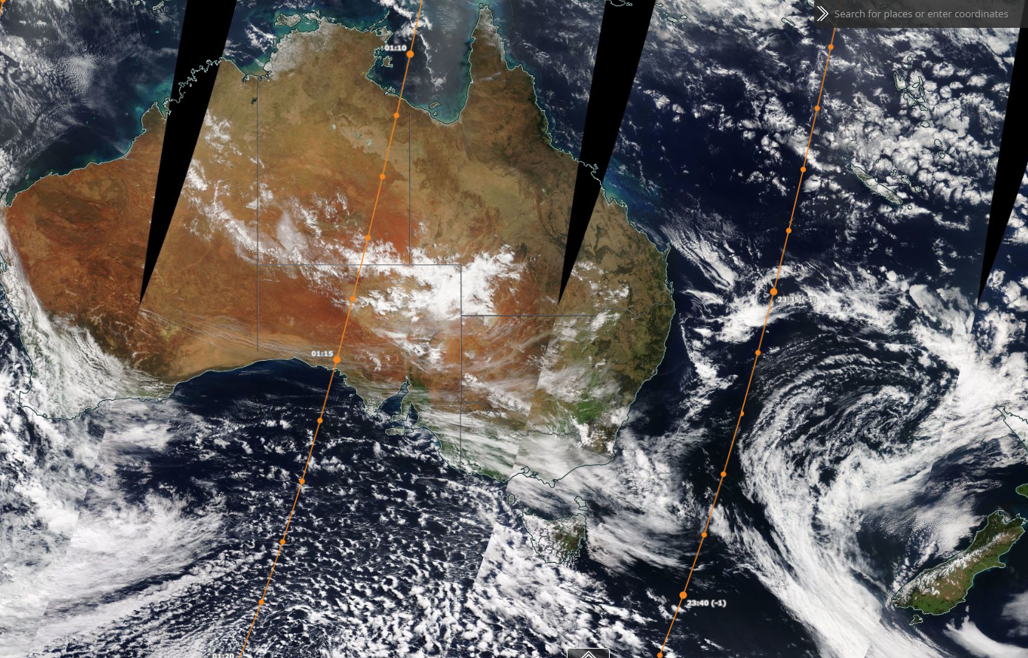
\includegraphics[width=\textwidth]{bilder/wrf/20T00_sat.png}
	\end{minipage}\hfill	
	\begin{minipage}[c]{0.35\textwidth}
		 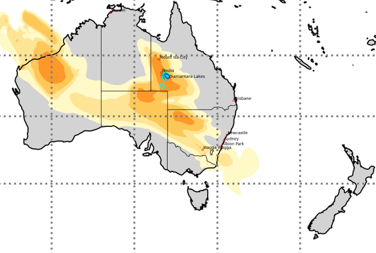
\includegraphics[width=\textwidth]{bilder/wrf/20T00_wrf.png}
	\end{minipage}\hfill
	\begin{minipage}[c]{0.29\textwidth}
		 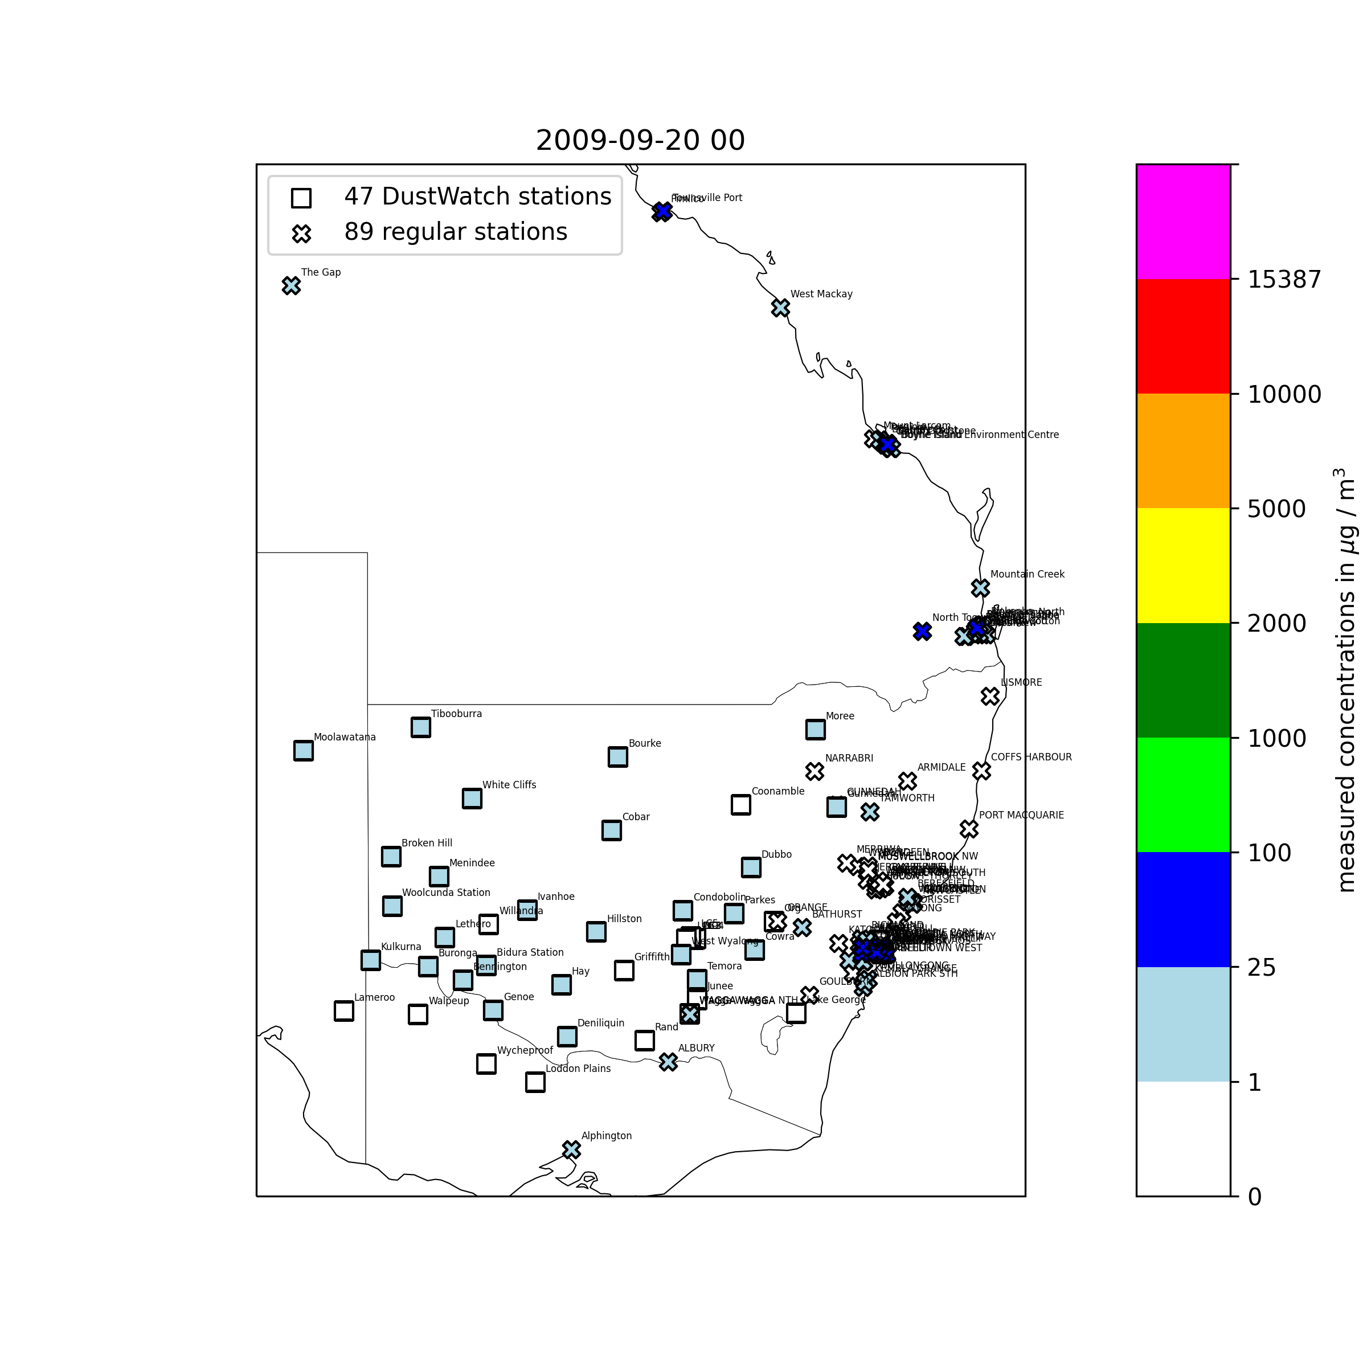
\includegraphics[width=\textwidth]{bilder/wrf/20T00_obs.png}
	\end{minipage}\hfill
	\begin{minipage}[c]{0.35\textwidth}
		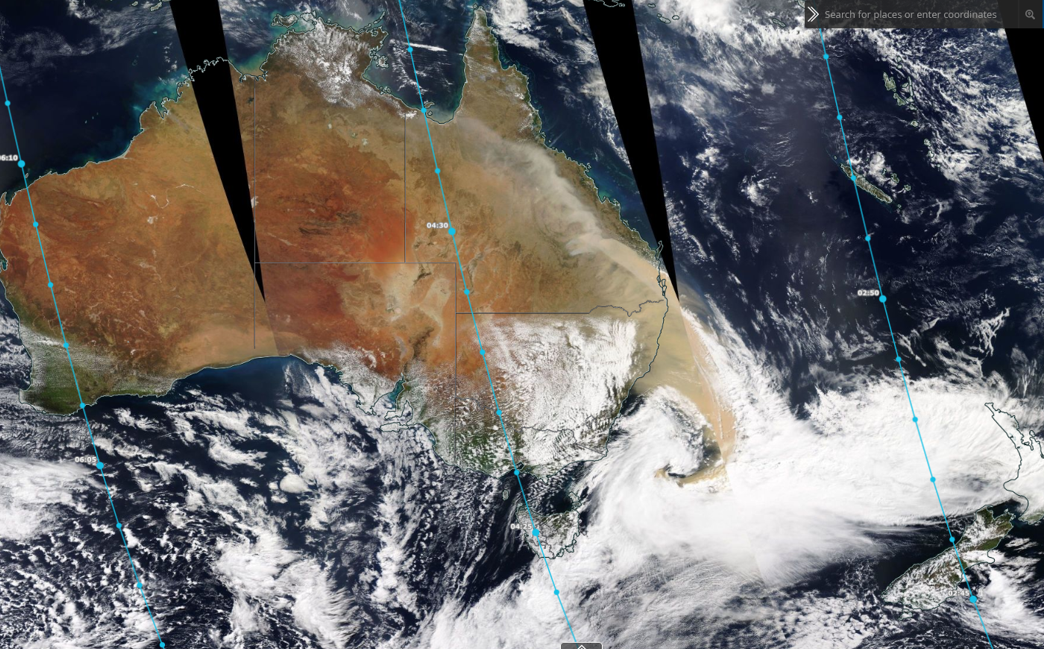
\includegraphics[width=\textwidth]{bilder/wrf/23T06_sat.png}
	\end{minipage}\hfill	
	\begin{minipage}[c]{0.35\textwidth}
		 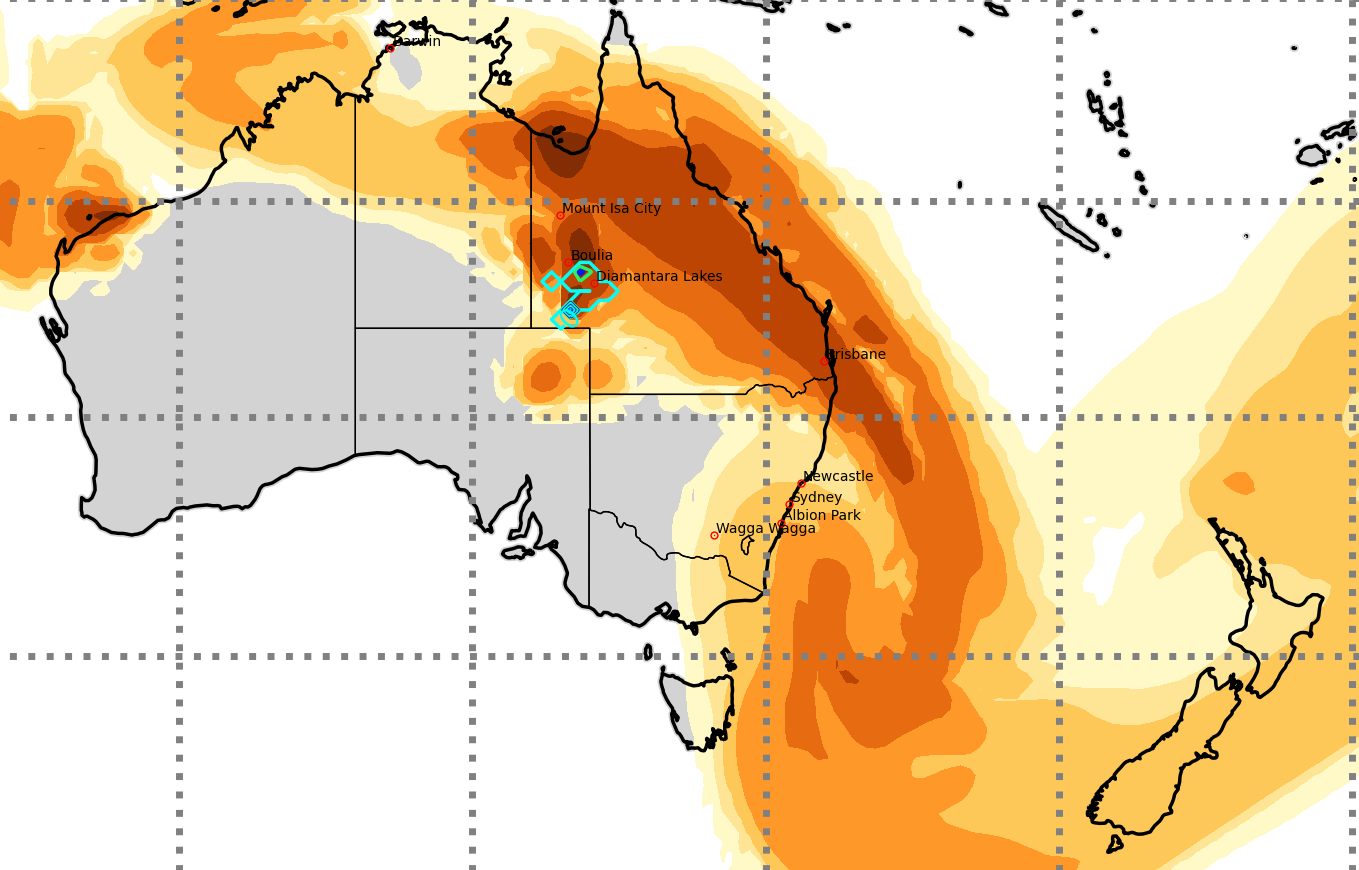
\includegraphics[width=\textwidth]{bilder/wrf/23T06_wrf.png}
	\end{minipage}\hfill
	\begin{minipage}[c]{0.29\textwidth}
		 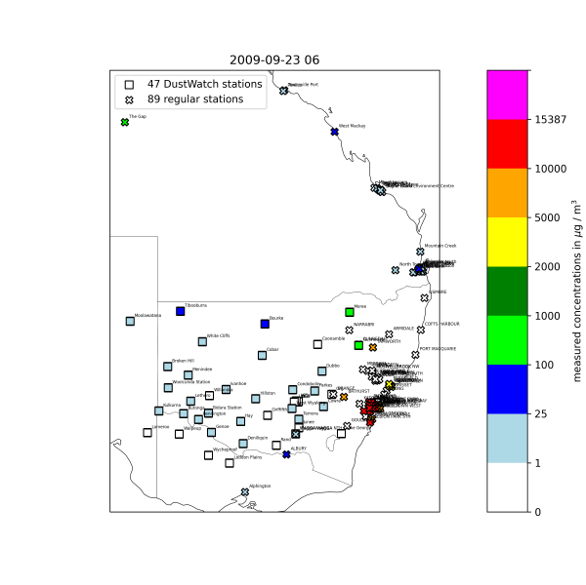
\includegraphics[width=\textwidth]{bilder/wrf/23T06_obs.png}
	\end{minipage}\hfill
	\begin{minipage}[c]{0.35\textwidth}
		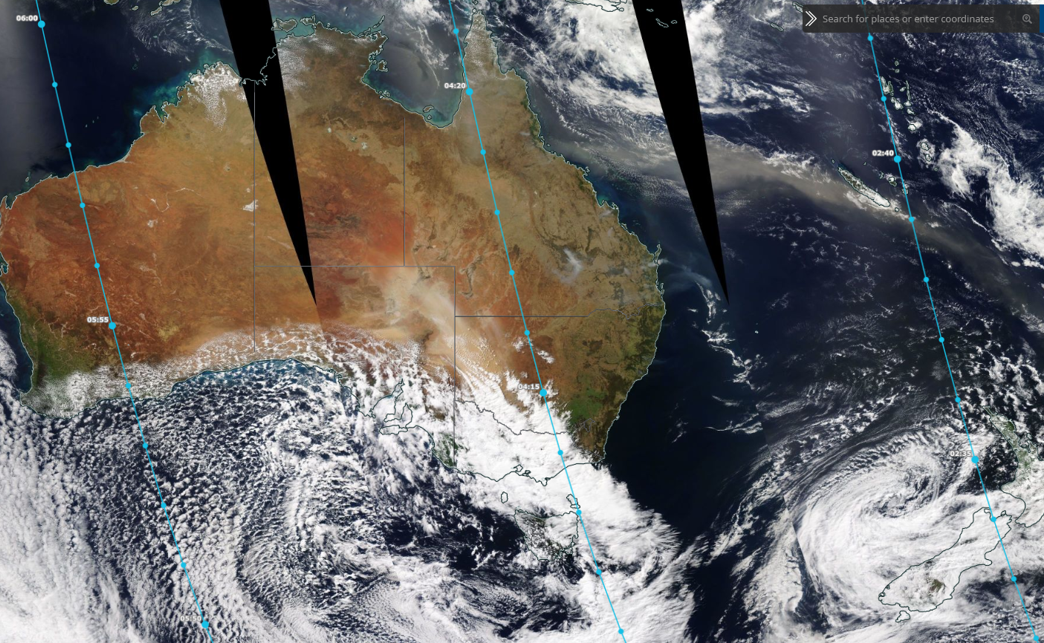
\includegraphics[width=\textwidth]{bilder/wrf/25T06_sat.png}
	\end{minipage}\hfill	
	\begin{minipage}[c]{0.35\textwidth}
		 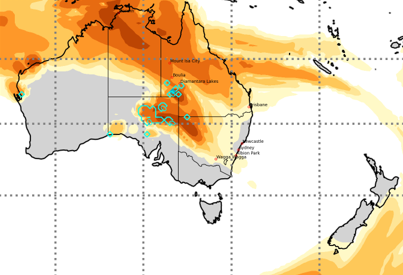
\includegraphics[width=\textwidth]{bilder/wrf/25T06_wrf.png}
	\end{minipage}\hfill
	\begin{minipage}[c]{0.29\textwidth}
		 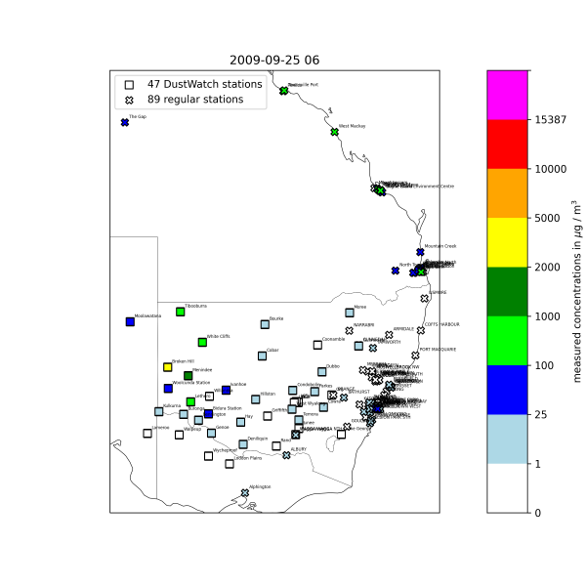
\includegraphics[width=\textwidth]{bilder/wrf/25T06_obs.png}
	\end{minipage}\hfill
	\begin{minipage}[c]{\textwidth}
		\captionsetup{format=hang, indention=0.0cm}
		\caption{Das muss ich irgendwie noch schöner machen....}
		\label{fig:wrf_sat}
	\end{minipage}
\end{figure}
Der Großteil des Staubs wird laut WRF-Modell aus der Region \textit{Channel Country} im Westen Queensland in der Nähe der \textit{Diamantina Lakes} emittiert. Diese Region wird grundsätzlich als Quelle für das Red-Dawn-Event vermutet (sh. Kapitel \textbf{XY}, \cite{Leys.2011}), allerdings bislang nicht als dominierende. Auf Abbildung \ref{fig:max_emis} wird deutlich, dass diese im Modell aber deutlich dominiert. Die Vermutung liegt nahe, dass ebendiese Emissionen zu den erhöhten (möglicherweise unrealistischen) modellierten Staubkonzentrationen im Nordwesten führen. Die Staubemissionen können im Modell aus verschiedenen Gründen überschätzt werden. Ein offensichtlicher Nachteil des im Modell implementierten Schemas zur Staubemission ist, dass nicht berücksichtigt wird, wie viel Staub am jeweiligen Gitterpunkt maximal emittiert werden kann. Ist eine Region also einmal als Staubquelle mit einer entsprechenden Größenordnung definiert, kann bei entsprechenden Windstärken theoretisch beliebig viel Staub emittiert werden. Dies soll in späteren Versionen durch eine \textit{Budgetierung} des maximal \textit{emissionsfähigen} Staubs an der Oberfläche implementiert werden, sodass die Emission stoppt, nachdem das Budget aufgebraucht ist. Durch neue Ablagerungen von Staub (Deposition) kann das Budget dann wieder aufgefüllt werden. Anschließend wären die Emissionen \textit{zeitlich} limitiert.
\begin{figure}[H]
\centering
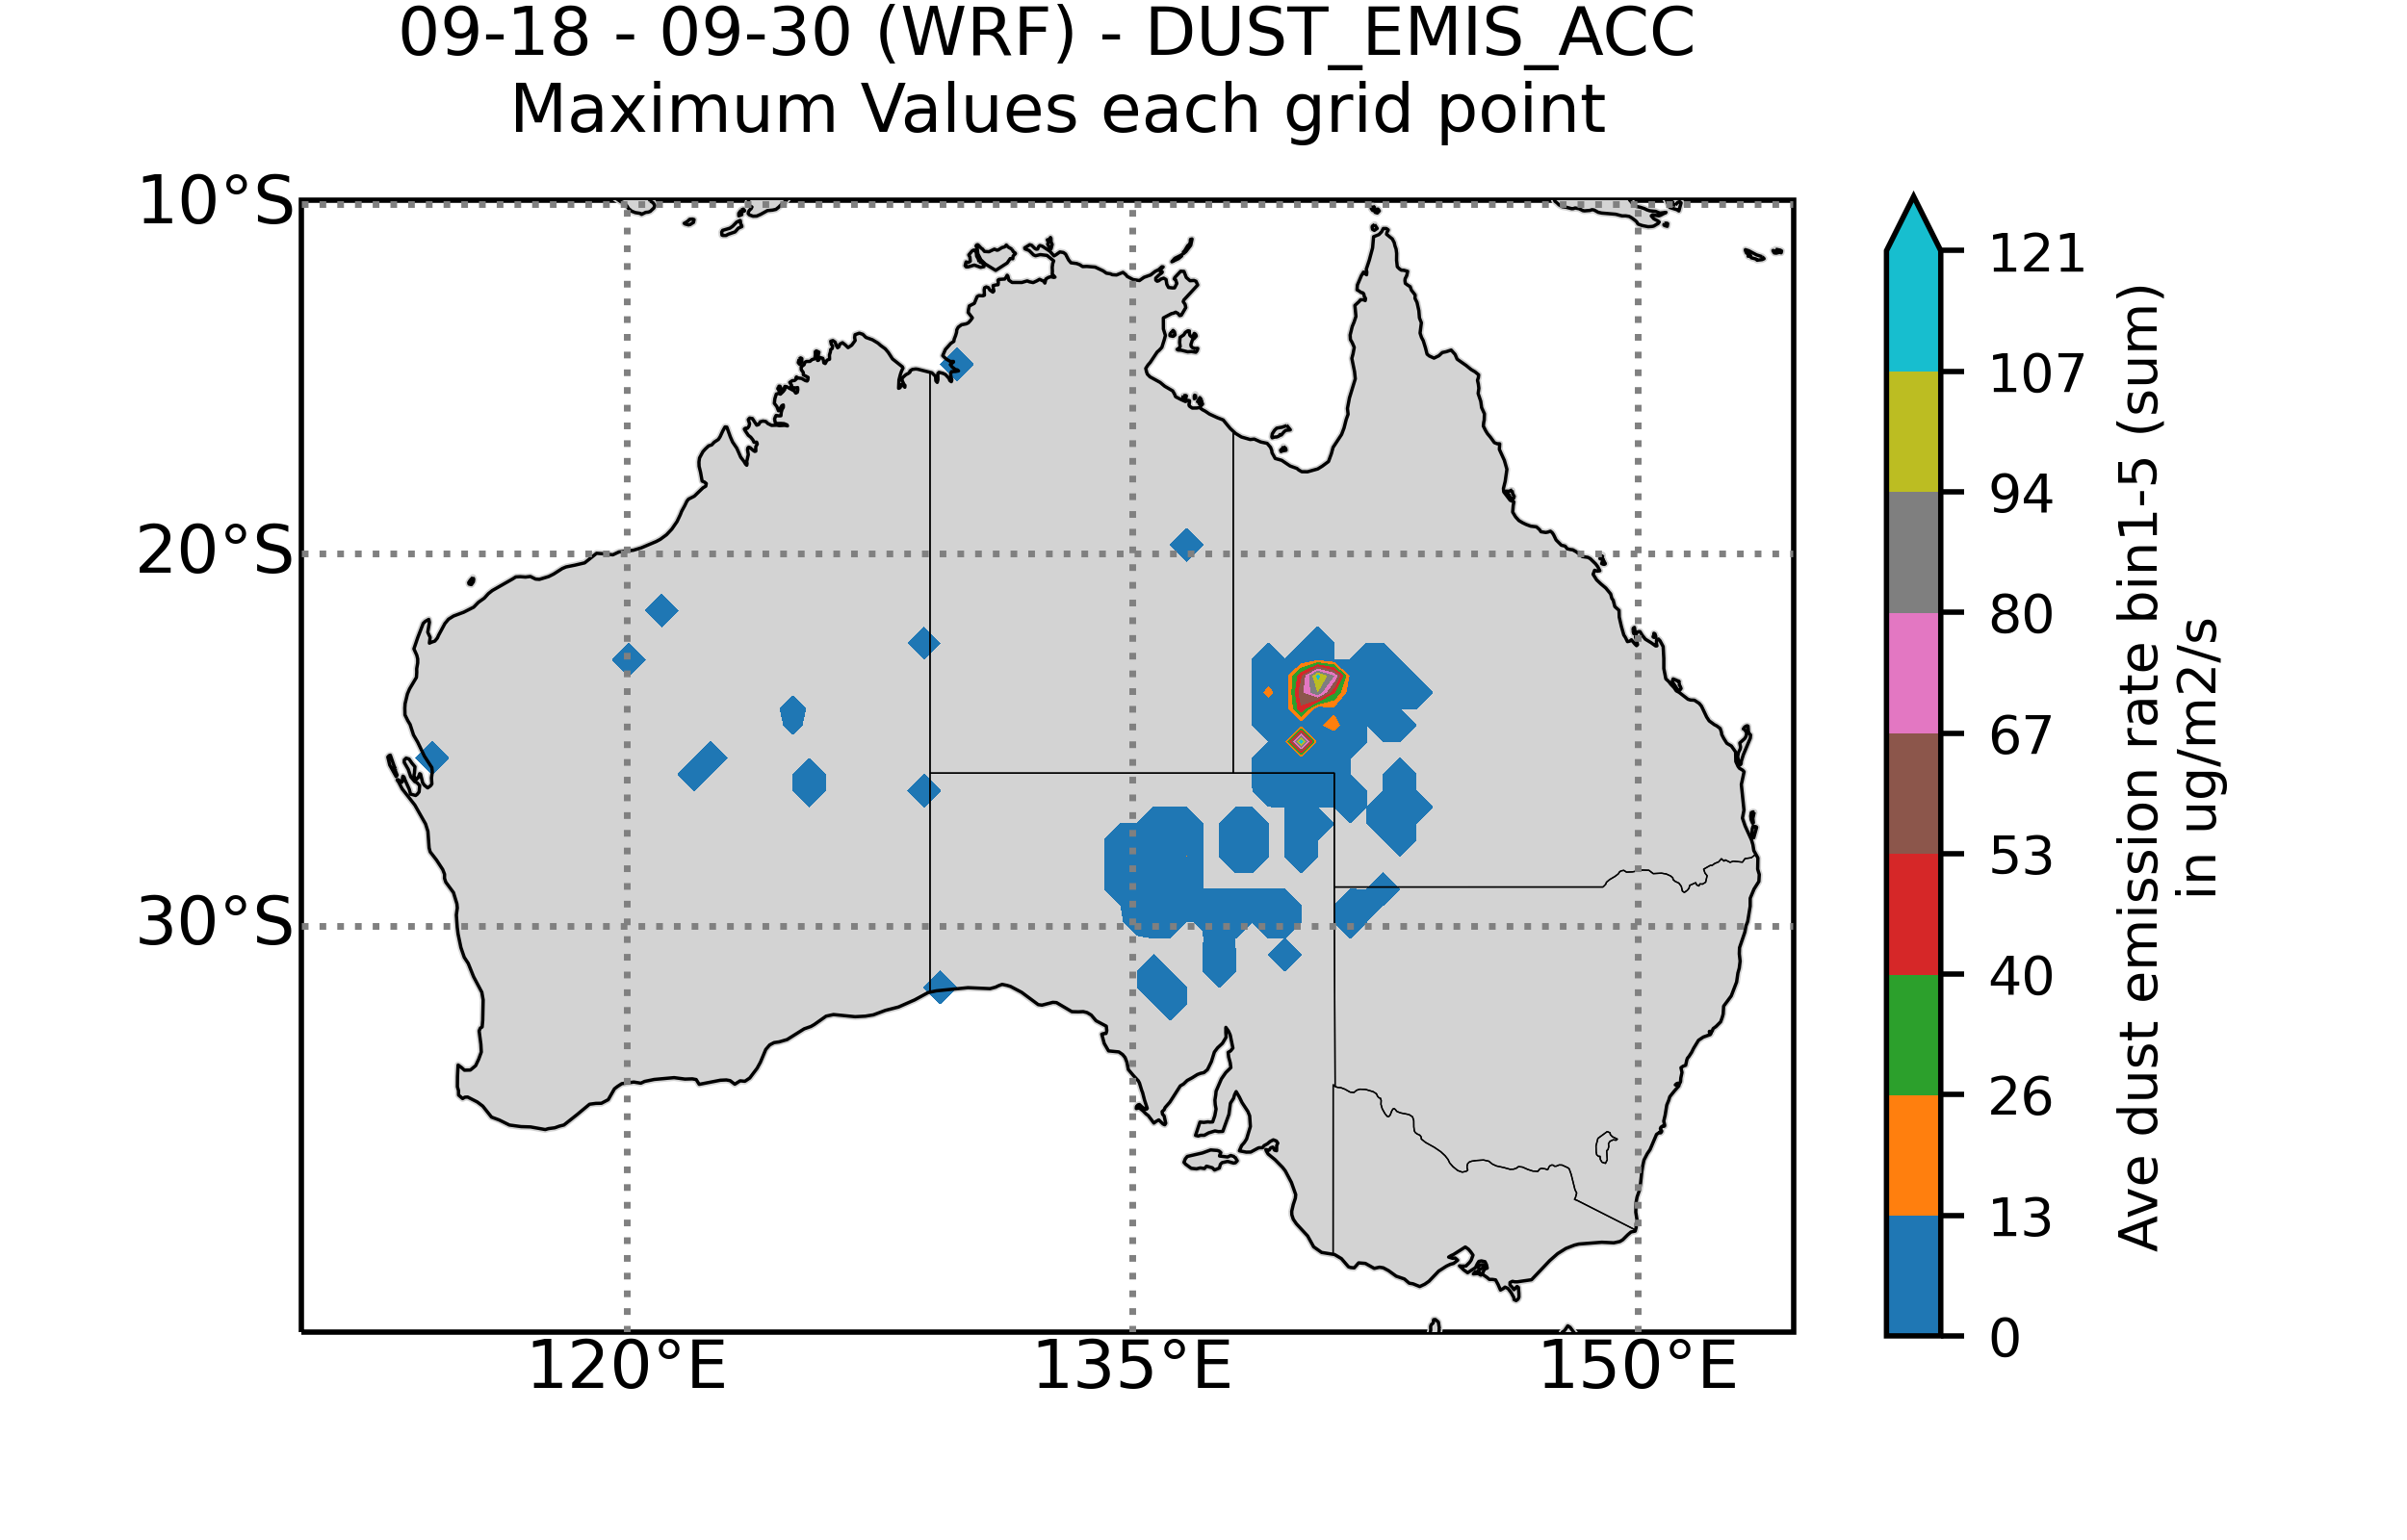
\includegraphics[width=\textwidth]{bilder/wrf/max_emis.png}
\caption{Darstellung der maximalen Staubemissionen über alle Zeiten je Gitterpunkt. Die Variablen DUST_EMIS_ACC1..5 beschreiben die über den letzten Zeitschritt (hier 3 Stunden) gemittelten Werte der Staubemissionen und wurden hier aufsummiert.} \label{fig:max_emis}
\end{figure}
Neben der zeitlichen Beschränkung beeinflussen verschiedene Parameter die zeitunabhängige Größenordnung der Emissionen. Insbesondere entscheidend für das Emissionspotential ist die Rauheit des Geländes. Dies stellt in Simulationen stets ein Problem dar, da die räumliche Auflösung eines diskreten Modells nie alle beliebig kleinen Elemente abdecken kann. Stattdessen wird jedem Gitterpunkt ein Parameter zugeordnet, der die Rauheit repräsentiert und die Emissionen stellvertretend regulieren soll. Im vorliegenden WRF-Modell werden dazu die Vegetationsparameter angepasst \textbf{LAI oder VEGFRA?}, da Vegetation einen vergleichbaren Einfluss nimmt wie Rauheit, bzw. ebenfalls eine gewisse Rauheit darstellt. Diese Informationen, welche Größe die Parameter an welchem Gitterpunkt annehmen, werden durch Geogrid-Daten in das WRF-Modell gegeben. In Abbildung \label{fig:emis_ctrl} sind einige der relevanten Parameter dargestellt. Es wird deutlich, dass die Zelle mit den höchsten Emissionen (\textit{1}) im Vergleich zu den Nachbarzellen etwas andere Werte erreicht, was zu verstärkten Emissionen führt. Da angenommen wird, dass die sehr hohen Emissionen unrealistisch sind, wurde der Blattflächenindex (LAI) an den 10 Gitterpunkten mit den höchsten Emissionen gezielt korrigiert. Dies führt zu einer veränderten Rauheit und soll die Emissionen auf ein adäquates Level limitieren.

\begin{figure}[H]
\centering
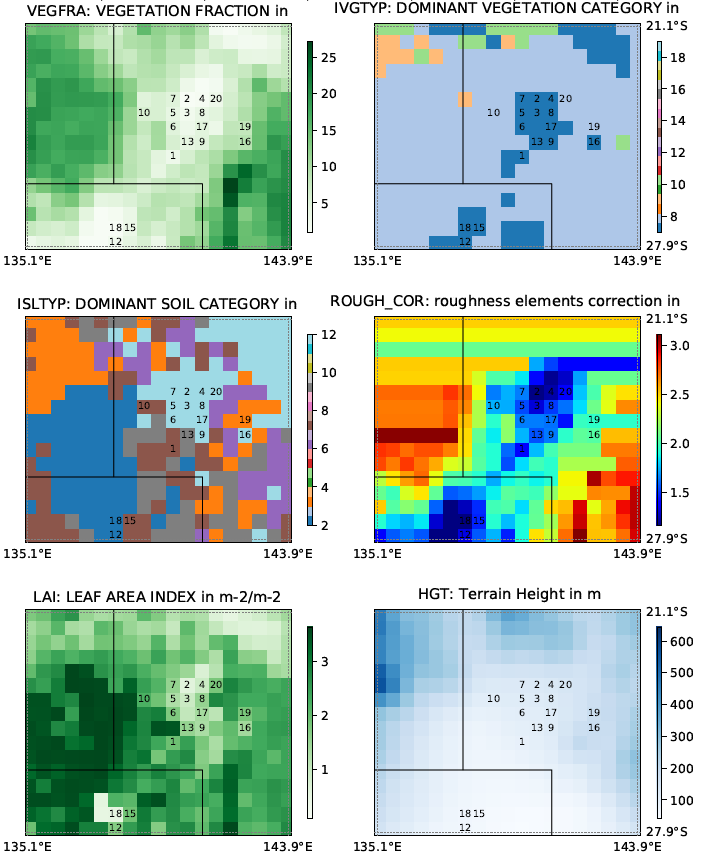
\includegraphics[width=0.7\textwidth]{bilder/wrf/emis_ctrl.png}
\caption{Absolute Werte einiger konstanter Parameter im WRF-Modell für die Region mit hohen Emissionen, die die Staubemissionen regulieren können. Die Zahlenwerte 1 bis 20 geben die Rangordnung der Staubemissionen an. Das heißt, Gitterpunkt 1 erreicht die höchste Emission, 2 die zweithöchste usw.}

\end{figure}



\subsection{Staubkonzentrationen}
- Hohe Konzentrationen an der Oberfläche werden durch Modell ungenügend beschrieben (siehe DUST_ACC_ auf zlevel 0 (geländefolgend)). DUSTLOAD über ganze Atmosphärensäule allerdings schon eher. Sehr sehr hohe Konzentrationen  ($>$ 10kg pro qm) später im Norden. 
\section{Staubquellen und Emissionen}
Laut Modell enorm hohe Emissionen zwischen Diamantara Lakes und Boulia (western Queensland). Laut \citet{Deckker.2019} konnte Lake Torrins als Quelle für Staub der bei Canberra gefallen ist identifiziert werden. Diese Region ebenfalls Bestandteil des Modells. Benutzt man die Unterteilung in \citet{OLoingsigh.2017}, dann laut Modell Region (2) Channel Country mit Abstand größte Quelle, aber auch (3) Lake Eyre (A) and South Simpson desert ephemeral lakes region, (4) South Strzelecki desert and Lake Frome (B) subbasin, (5) Lakes Torrens (C).
\section{Zusammenfassung und Ausblick}
\newpage
\printbibliography
\newpage
\appendix
\section{Anhang}
\addcontentsline{toc}{section}{Abbildungsverzeichnis}
\listoffigures
\addcontentsline{toc}{section}{Tabellenverzeichnis}
\listoftables
\section{Danksagung}
\end{document}
